% ====================================================================
%+
% SECTION:
%    SolarSystem_CometActivity.tex
%
% CHAPTER:
%    solarsystem.tex
%
% ELEVATOR PITCH:
%-
% ====================================================================

\section{Detecting Comet Activity}
\def\secname{\chpname:activity}\label{sec:\secname}

\credit{rhiannonlynne},
\credit{davidtrilling},
\credit{migueldvb}

Comets are the remnant building blocks of the Solar System
that have been stored at cold temperatures beyond the ice
line, either in the Kuiper belt or the Oort cloud, since their
formation.  Measuring the evolution of cometary activity over
a range of heliocentric distances with LSST will allow us to
understand the overall comet activity and to link these
observations with the physical and chemical conditions in the
early solar nebula during planet formation.  Comets are
classified in two main dynamical families, Jupiter Family
comets (JFCs) that have low-inclination orbits with periods
less than 20 years, and Long-period comets (LPCs) that
originate in the Oort Cloud at a distance of more than 10000
AU and have large orbital eccentricities and nearly isotropic
distribution of inclinations.  Currently there are over 400
Jupiter-family comets known, most of which are faint compared
with the LPCs.  LSST will observe about $10^4$ individual
comets repeatedly including measurements of known objects over
its 10-year survey \citep{2010PhDT.......241S}. The
determination of their activity levels at various heliocentric
distances will be used to study the time evolution of each
object individually and to find the connection between comet
families and their formation region in the Solar System.

Several cometary volatiles result in strong emission bands
excited by solar radiation that emit by resonant fluorescence
at optical and near-ultraviolet wavelengths.  The LSST $u$
filter peaks near the CN (0--0) emission band at 3880 \r{A}.
Although CN is not the most abundant daughter species from
cometary volatiles and the OH (0--0) emission band at 3080
\r{A} is generally stronger, CN production rates provide an
excellent proxy of the level of overall gas activity in
comets. LSST will offer a unique opportunity to produce
a large database of CN production rates, vastly increasing our current
knowledge \citep[see
e.g.][]{1995Icar..118..223A, 2012ApJ...758...29A}.
 Other bands such as $r$, $i$, and $z$ will detect
continuum brightness that is produced by reflected radiation
from dust particles in the coma. Thus, it will be possible to
obtain the evolution of the gas-to-dust production ratio at
high cadence as a function of heliocentric distance in
different comet families. The greatly increased sample size
compared with previous catalogs \citep{1995Icar..118..223A}
will allow for statistical comparison of the comet families
and to link them to other small body populations in the Solar
System.

A recently discovered population of main-belt asteroids eject
dust and produce coma and tails giving them the appearance of
comets \citep{2012AJ....143...66J}.  This so-called main-belt
comets or active asteroids have the orbital characteristics of
asteroids with $T_J > 3$ and lose mass during part of their
orbits. The cometary activity observed in these objects may be
driven by primordial water water ice that is trapped near the
surface and sublimates when it is exposed to sunlight.
Main-belt comets are important because they may have been able to
preserve water ice despite the effect of solar radiation and
heating from the decay of short-lived radioactive nuclei.  The
asteroids in the outer regions of the main belt can therefore
have a substantial fraction of water and other volatiles that
may have supplied the volatile content of terrestrial planets.
Most of the main-belt-comets are faint with very weak comae
that are active during part of their orbits. Given the
expected flux sensitivity of LSST, the transient cometary
activity of main-belt asteroids will be observable including
many objects that could be below the detection limits of
current photometric surveys.  The LSST observations will thus
help to understand the overlap between different populations
in the Solar System such as the relationship between comets
and asteroids.

% --------------------------------------------------------------------

\subsection{Target measurements and discoveries}
\label{sec:\secname:targets}

LSST will make an exceptionally large number of comet
observations.  About $10^4$ comets will be observed on average
of 50 times by LSST during its main survey, while a few objects
will be observed more than 1000 times
\citep{2010PhDT.......241S}.  Simulations of characteristic
comet orbits have shown that LSST will observe some Jupiter
Family comets (JFCs) hundreds of times over their full orbits
\citep{2010PhDT.......241S}.  Individual LPCs are predicted to
be observed by LSST with dozens of observations as they
approach or recede from the center of the Solar System or
during their perihelion passage.  Thus, these observations
will trace the onset of outgassing from quiescence at large
heliocentric distances and the decline of activity after
perihelion.

Ensuring that any activity or outgassing of a comet or active asteroid
is clearly identifiable with LSST DM or contributed Level 3 software is not a
solved problem, however there is ongoing work toward this goal (xx
ref? Hsieh, other? xx). In the meantime, it does not seem unreasonable
to assume that the main requirement, in terms of cadence, is to actually
have an observation at a time when activity is visible, as well as at
surrounding times to determine the start and end points of that activity.

Cometary activity and outgassing can last for various periods of time,
usually on the order of days to weeks. It can be transient, perhaps
due to a collision or other resurfacing event, or it can be periodic,
such as repeated activity when an object approaches perihelion. Thus,
in order to characterize the fraction of active asteroids, or to
understand the causes of their activity, or to understand cometary
activity as a function of source population (and thus presumably
composition) and heliocentric distance, the goal would be to have
repeated observations spread throughout the period when the object is visible.


% --------------------------------------------------------------------

\subsection{Metrics}
\label{sec:\secname:metrics}

A full exploration of the cadence effects on measuring activity rates
for comets and active asteroids would include understanding the
selection effects of when the object was not observed, as well as the
likelihood of detecting activity based on when it was observed. For
now, we have focused on the likelihood of being able to detect
activity lasting a given amount of time.

The metrics {\tt ActivityOverTimeMetric} and {\tt
  ActivityOverPeriodMetric} look at when an object was observed (with
a detection above a given SNR), and
split those observations into bins based on time or position in the
orbit (mean anomaly), respectively. The first is relevant when looking
for transient activity that is not expected to repeat at the same
point in the orbit, while the second seems more appropriate for
activity that would repeat at the same point in the orbit. Each of
these metrics takes only a single time or mean anomaly window, distributes
the observations of each object into bins based on those windows, and
counts the number of bins which received observations. The number of
bins with observations, compared to the overall number of bins,
determines the calculated likelihood of detecting activity for that
object.

To investigate the sensitivity of LSST to activity on a range of
timescales and lasting various fractions of the period, we ran these
metrics over a range of values and then plot the minimum, mean, and
maximum likelihoods of objects at a particular $H$ value, for various populations.


% --------------------------------------------------------------------

\subsection{OpSim Analysis}
\label{sec:\secname:analysis}

Running these metrics on a sample Main Belt Asteroid population
generates results illustrated in Figure~\ref{activity}.
In the baseline survey \opsimdbref{db:baseCadence}, the metric results
indicate that for bright asteroids with activity lasting more than
about 60 days, we have between about 18-60\% chance of obtaining at
least one observation that captures the event. If the activity is
periodic, and lasts around 10\% of the orbit, we have between
20-65\% chance of observing the activity. If the periods of activity
last longer, we have a higher chance of having an observation which
captures that activity, as expected.

That the chance of detecting activity is not significantly higher for
repeating events than for transient events is interesting. It's not
clear if this reflects a characteristic of the observing cadence
(e.g.\ perhaps the observations always are clustered near the same
point in the orbit, leaving many ``bins'' unwatched), but it's seems
likely that at  the very least, the metric should be tuned to account for the additional
likelihood of activity occurring near perihelion.

\begin{figure}
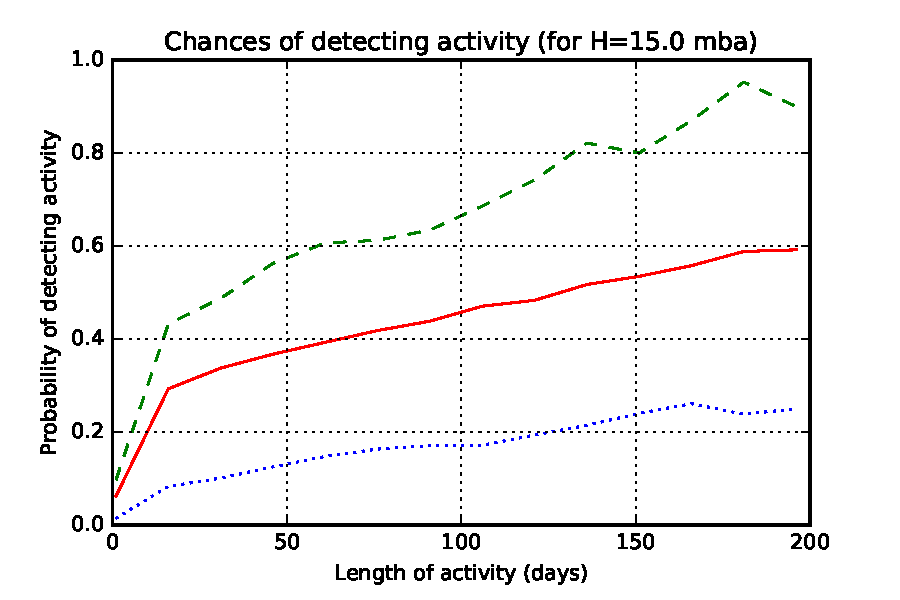
\includegraphics[width=3.3in]{figs/solarsystem/minion_1016_mba_Activity_time}
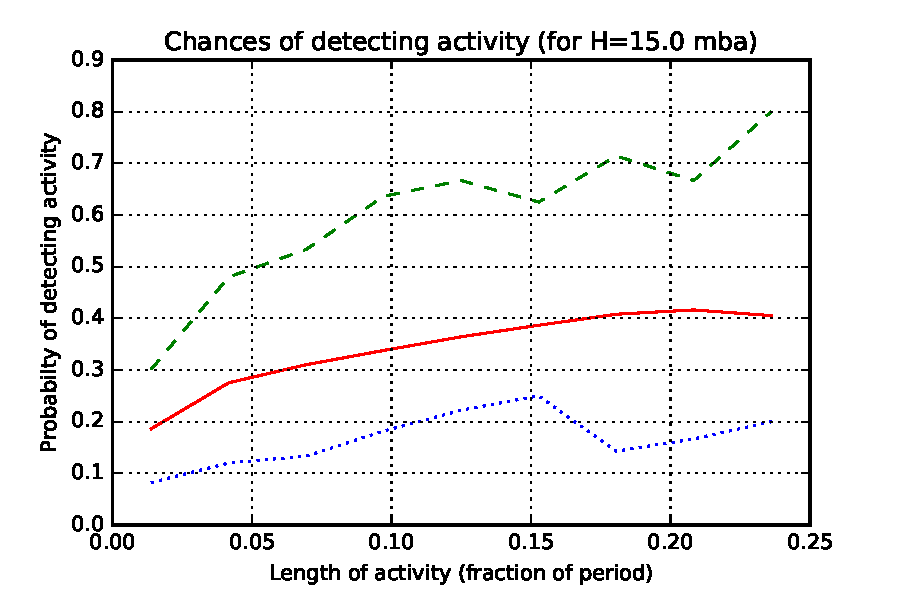
\includegraphics[width=3.3in]{figs/solarsystem/minion_1016_mba_Activity_period}
\caption{Likelihood of detecting activity or outgassing for MBAs, for
  a single event lasting a given number of days (left) or an event
  potentially repeating for a given fraction of the period (right).
\label{activity}}
\end{figure}


% --------------------------------------------------------------------

\subsection{Discussion}
\label{sec:\secname:discussion}

The likelihood of detecting activity depends on if the observing
strategy is such that we observe an object when it is active, and the
capability to identify this activity in the acquired images.

In terms of observing strategy, if observations are clumped together
irregularly in time, we risk missing activity during the times we do
not observe the object, although with the possible benefit of being
more likely to detect short time-scale activity during the times we
have more frequent observations. Balancing these two tensions likely
requires more knowledge about the relevant timescales for activity on
active asteroids, as only a handful of active asteroids have currently
been identified. (comment on cometary activity?)

% --------------------------------------------------------------------

\navigationbar
